\documentclass[10pt,letterpaper]{article}
\usepackage[utf8]{inputenc}
\usepackage[margin=1in]{geometry}
\usepackage{amsmath}
\usepackage{amsfonts}
\usepackage{amsthm}
\usepackage{mathtools,amssymb}
\usepackage{amssymb}
\usepackage{float}
\usepackage{graphicx}
\numberwithin{table}{section}
\numberwithin{figure}{section}
\numberwithin{equation}{section}
\usepackage{varioref}
\labelformat{euqation}{(#1)}
\usepackage[colorlinks]{hyperref}
\usepackage{bm}
\usepackage{listings}
\usepackage[]{algorithm2e}
\renewcommand{\qedsymbol}{\rule{0.7em}{0.7em}}
%\usepackage[singlelinecheck=false]{caption}
% new command
\newcommand{\beq}{\begin{equation}}
\newcommand{\eeq}{\end{equation}}
\newcommand{\bs}{\begin{split}}
\newcommand{\es}{\end{split}}
\newcommand{\bct}{\begin{center}}
\newcommand{\ect}{\end{center}}
\newenvironment{centergroup}{\trivlist\item\begin{minipage}{\columnwidth}\centering}{\end{minipage}
\endtrivlist}

\newcommand\independent{\protect\mathpalette{\protect\independenT}{\perp}}
\def\independenT#1#2{\mathrel{\rlap{$#1#2$}\mkern2mu{#1#2}}}



\title{Accounting for Uncertainty in Percolation Regimes}
\author{Xiaojing Zhu}

\begin{document}
\maketitle

\section{Continuous-time ER Process}
\subsection{Model Defination (noise-free)}
Let 
\begin{equation}
\{G(t)= (V, E(t)), t_1 \leq t\leq t_M\}
\end{equation}
be a continous-time ER process, where $G(t)$ is the undirected graph, $V$ is the vertex set of $G(t)$ (unchanged), and $E(t)$ is the edge set at time $t$. 

The network $G(t)$ can be identified with its $n \times n$ adjacency matrix: $Y(t) \in R^{N \times N}$, with $Y_{ij}(t) = 1/0$, $|V| = N$. Hence, the continous-time ER process can be represented as 
\begin{equation}
\{Y(t) \in R^{N \times N}, t_1 \leq t\leq t_M\}
\end{equation}

[Wes Wiles] Such a sequence will be said to be Markov if its edge sets are controlled by a Markov chain. We impose this dependence through the use of binary random variable, denoted $\{W(t) \in \{0,1\}, t_1\leq t \leq t_M\}$. The continuous-time ER process, which is now the network-valued Markov chain, can therefore be represented as 
\begin{equation}
\{(Y(t),W(t)) \in R^{N \times N} \times \{0,1\}, t_1 \leq t\leq t_M\}
\end{equation}

The continuous-time ER process can be specified as follows: 
\begin{enumerate}


\item Transition Time:\\
Assume that at any time point $t$ with $Y(t) = y$, the waiting time until the next edge change is exponential distributed with rate parameter $ \lambda (\gamma, y)$, (three options proposed here) 
\begin{equation}
 \lambda (\gamma, y) = \gamma 
\end{equation}
or
\begin{equation}
 \lambda (\gamma, y) =  \lambda (\gamma, t) = \exp (\sum_{k=1}^L \gamma_k Z_k(t)) 
\end{equation}
where $Z_k(t)$'s are the covariates recorded at time $t$. \\
or 
\begin{equation}
 \lambda (\gamma, y) =  \lambda (\gamma, t) = \exp (\sum_{k=1}^L \gamma_k r_k(y)) 
\end{equation}
where $r_k(y)$'s are some functions/characteristics of the current network $y$. 

\item Options for change \\
For two consecutive transition time points $\tau_1, \tau_2$, the network $Y(\tau_2)$ differs from $Y(\tau_1)$ by a single edge, and the edge is chosen to be added or deleted at random with prob. $p$ (or $1-q$) or $1-p$ (or $q$), depending on the binary variable $W(\tau_1), W(\tau_2)$ (Table \ref{tab1.1}, \ref{tab1.2}, \ref{tab1.3}), i.e. we have 
\begin{equation}
\begin{split}
Y_{ij}(\tau_2) &\neq Y_{ij}(\tau_1) \text{ for one pair of } (i, j), i \neq j, \\
Y_{ij}(\tau_2) &= Y_{ij}(\tau_1)  \text{ for other } (i, j)
\end{split}
\end{equation}

\begin{table}[H]
\centering
\begin{tabular}{lll}
\hline
 &  $W(\tau_2)=0$&  $W(\tau_2)=1$\\\hline
$W(\tau_1)=0$ &  $1-p$ &  $p$\\
$W(\tau_1)=1$ &  $q$ & $1-q$\\\hline
\end{tabular}
\caption{ER transition probability matrix for $W(t)$ at two consecutive transition time $(\tau_1, \tau_2)$, $\tau_1 < \tau_2$, when $Y(\tau_1)$ is neither empty or complete}
\label{tab1.1}
\end{table}

\begin{table}[H]
\centering
\begin{tabular}{lll}
\hline
 &  $W(\tau_2)=0$&  $W(\tau_2)=1$\\\hline
$W(\tau_1)=0$ &  $0$ &  $1$\\
$W(\tau_1)=1$ &  $0$ & $1$\\\hline
\end{tabular}
\caption{ER transition probability matrix for $W(t)$ at two consecutive transition time $(\tau_1, \tau_2)$, $\tau_1 < \tau_2$, when $Y(\tau_1)$ is empty}
\label{tab1.2}
\end{table}

\begin{table}[H]
\centering
\begin{tabular}{lll}
\hline
 &  $W(\tau_2)=0$&  $W(\tau_2)=1$\\\hline
$W(\tau_1)=0$ &  $1$ &  $0$\\
$W(\tau_1)=1$ &  $1$ & $0$\\\hline
\end{tabular}
\caption{ER transition probability matrix for $W(t)$ at two consecutive transition time $(\tau_1, \tau_2)$, $\tau_1 < \tau_2$, when $Y(\tau_1)$ is complete}
\label{tab1.3}
\end{table}

\item Transition Probability \\
By the definition of ER process, we can see that the probability that the network changes from $y_1$ to $y_2$ in a single step is 
\begin{equation}
\label{1.8}
P(Y(\tau_2) = y_2|Y(\tau_1) = y_1) 
= \begin{cases}
0 \quad \text{ if } y_1, y_2 \text{ differ by more than 1 pair of } (i,j) \text{ or }y_1, y_2 \text{ are the same} \\
P(Y_{ij}(\tau_2) = 1 (or 0)|Y_{ij}(\tau_1) = 0 (or 1)) \quad \text{ if } y_1, y_2 \text{ differ by only one } (i,j). \\
\end{cases} 
\end{equation}
where 
\begin{equation}
P(Y_{ij}(\tau_2) = 1|Y_{ij}(\tau_1) = 0) = 
\begin{cases}
\frac{p}{\# \text{non-edges in}Y(\tau_1)} \text{  if  }  W(\tau_1) = 0 \\
\frac{1-q}{\# \text{non-edges in}Y(\tau_1)} \text{  if  } W(\tau_1) = 1 \\
\end{cases}
\end{equation}
(not include boundary cases here)
\begin{equation}
P(Y_{ij}(\tau_2) = 0|Y_{ij}(\tau_1) = 1) = 
\begin{cases}
\frac{1-p}{\# \text{edges in}Y(\tau_1)} \text{  if  }  W(\tau_1) = 0 \\
\frac{q}{\# \text{edges in}Y(\tau_1)} \text{  if  } W(\tau_1) = 1 \\
\end{cases}
\end{equation}
(not include boundary cases here)

Notice that 
\begin{equation}
\label{1.11}
P(Y_{ij}(\tau_2) = 1|Y_{ij}(\tau_1) = 0) = 
\begin{cases}
\frac{1}{\# \text{none-dges in}Y(\tau_1)} \text{  if  } W(\tau_2) = 1 \\
0 \text{  if  }  W(\tau_2) = 0 
\end{cases}
\end{equation}

\begin{equation}
\label{1.12}
P(Y_{ij}(\tau_2) = 0|Y_{ij}(\tau_1) = 1) = 
\begin{cases}
\frac{1}{\# \text{edges in}Y(\tau_1)} \text{  if  }  W(\tau_2) = 0 \\
0\text{  if  } W(\tau_2) = 1 \\
\end{cases}
\end{equation}

$\Rightarrow$ the distribution of $W(\tau_2)|W(\tau_1), Y(\tau_1)$ is known

$\Rightarrow$ the ditribution of $Y(\tau_2)|Y(\tau_1)$ conditional on $W(\tau_1)$ or $W(\tau_2)$ is known, i.e.\\
$Y(\tau_2)|Y(\tau_1), W(\tau_1)$ and  $Y(\tau_2)|Y(\tau_1), W(\tau_2)$ are known

\end{enumerate} 

%%%%%%%%%%%%%
\fbox{
\parbox{1\linewidth}{
The transition probability for the network-valued Markov chain, $\{\big(Y(t),W(t)\big)\in R^{N\times N} \times \{0,1\}, t_1\leq t \leq t_M\}$, from $(y_1,w_1)$ to $(y_2,w_2)$ in a single step is 

\iffalse
\begin{equation}
\begin{split}
&p \Big(
\big(Y(\tau_2),W(\tau_2)\big) = \big(y(\tau_2),w(\tau_2)\big)|\big(Y(\tau_1), W(\tau_1)\big)  =  \big(y(\tau_1),w(\tau_1)\big) 
\Big)\\
&= p\Big(
Y(\tau_2)=y(\tau_2),W(\tau_2) = w(\tau_2)|Y(\tau_1) = y(\tau_1),W(\tau_1) = w(\tau_1)
\Big) \\
&= p\Big(
Y(\tau_2)=y(\tau_2)|W(\tau_2)=w(\tau_2),Y(\tau_1)=y(\tau_1),W(\tau_1)=w(\tau_1)
\Big) 
\cdot
p\Big(
W(\tau_2)=w(\tau_2)|Y(\tau_1)=y(\tau_1),W(\tau_1)=w(\tau_1)
\Big) \\
&= p\Big(
Y(\tau_2)=y(\tau_2)|W(\tau_2)=w(\tau_2),Y(\tau_1)=y(\tau_1)
\Big) 
\cdot
p\Big(
W(\tau_2)=w(\tau_2)|Y(\tau_1)=y(\tau_1),W(\tau_1)=w(\tau_1)
\Big) \\ 
&\qquad \text{since }Y(\tau_2) \independent W(\tau_{1}) | Y(\tau_{1}), W(\tau_{2})
\\
\end{split}
\end{equation}
\fi

\begin{equation}
\begin{split}
&P \Big(
\big(Y(\tau_2),W(\tau_2)\big) = \big(y_2,w_2\big)|\big(Y(\tau_1), W(\tau_1)\big)  =  \big(y_1,w_1\big) 
\Big)\\
&= P\Big(
Y(\tau_2)=y_2,W(\tau_2) = w_2|Y(\tau_1) = y_1,W(\tau_1) = w_1
\Big) \\
&= P\Big(
Y(\tau_2)=y_2|W(\tau_2)=w_2,Y(\tau_1)=y_1,W(\tau_1)=w_1
\Big) 
\cdot
P\Big(
W(\tau_2)=w_2|Y(\tau_1)=y_1,W(\tau_1)=w_1
\Big) \\
&= P\Big(
Y(\tau_2)=y_2|W(\tau_2)=w_2,Y(\tau_1)=y_1
\Big) 
\cdot
P\Big(
W(\tau_2)=w_2|Y(\tau_1)=y_1,W(\tau_1)=w_1
\Big) \\ 
&\qquad (\text{since }Y(\tau_2) \independent W(\tau_{1}) | Y(\tau_{1}), W(\tau_{2}))\\
\end{split}
\end{equation}
where $\tau_1,\tau_2$ are two arbitrary consecutive transition time points, $\tau_1<\tau_2$. The first probability is given in \ref{1.8}, \ref{1.11}, \ref{1.12}, and the second probability is given in Table \ref{tab1.1}, \ref{tab1.2}, \ref{tab1.3}.
\\~\\
We can rewrite the transition probability with pdfs as 
\begin{equation}
\label{1.14}
f(y_2,w_2|y_1,w_1) = g (y_2|w_2,y_1) \cdot h(w_2|y_1,w_1)
\end{equation}
where $f(\cdot|\cdot)$ is the conditional pdf of rvs $\big(Y(\tau_2),W(\tau_2)\big)$ given $\big(Y(\tau_1),W(\tau_1)\big)$, $g(\cdot|\cdot)$ is the conditional pdf of rv. $Y(\tau_2)$ given $\big(W(\tau_2), Y(\tau_1)\big)$, and $h(\cdot|\cdot)$ is the conditional pdf of rv. $W(\tau_2)$ given $\big(Y(\tau_1), W(\tau_1)\big)$. $\tau_1,\tau_2$ are two arbitrary consecutive transition time points, $\tau_1<\tau_2$.
\\~\\
Specifically, 
\begin{equation}
g(y_2|w_2,y_1) = ... \text{doesn't depend on } p,q,\gamma
\end{equation}
\begin{equation}
\begin{split}
h(w_2|y_1,w_1) & = h_{p,q}(w_2|y_1,w_1) \\
& = w_2 \bm 1_{\{y_1 = \text{Empty} \}} + 
(1-w_2) \bm 1_{\{y_1 = \text{Complete} \}} + \\
&
\big(p^{w_2}(1-p)^{1-w_2} \bm 1_{\{w_1 = 0 \}} +
      (1-q)^{w_2}q^{1-w_2}  \bm 1_{\{w_1 = 1 \}}
 \big)
\bm 1_{\{y_1 \neq \text{Empty or Complete}  \}}
\end{split}
\end{equation}
}
}


\iffalse
\begin{equation}
\begin{split}
&p \Big(
\big(Y(\tau_2),W(\tau_2)\big) = \big(y(\tau_2),w(\tau_2)\big)|\big(Y(\tau_1), W(\tau_1)\big)  =  \big(y(\tau_1),w(\tau_1)\big) 
\Big)\\
&= p(y(\tau_2),w(\tau_2)|y(\tau_1),w(\tau_1)) \\
&= p(y(\tau_2)|w(\tau_2),y(\tau_1),w(\tau_1)) \cdot
p(w(\tau_2)|y(\tau_1),w(\tau_1)) \\
& = p(y(\tau_2)|w(\tau_2),y(\tau_1)) \cdot
p(w(\tau_2)|y(\tau_1),w(\tau_1))   \qquad \text{since }Y(\tau_2) \independent W(\tau_{1}) | Y(\tau_{1}), W(\tau_{2})
\\
\end{split}
\end{equation}
\fi 

\subsection{Observing Snapshots}
Assume that we have $M$ observations $[y(t_1), y(t_2),...,y(t_M)]$ on the stochastic process of network with $N$ nodes, where $t_1< t_2,...,<t_M$ are the observation moments. 
%where $t_m^{-}$ represents the most recent transitioning time happened up to observational time $t_m$. 
Given such samples at discrete-time, for the continuous-time probability model $\{\big(Y(t),W(t)\big), t_1 \leq t\leq t_M\}$, there is no closed-form for the marginal distribution of snapshots. Instead of considering log-likelihood for observed data, we consider the log-likelihood for augmented data. 


\subsubsection{Augmented data}
The data augmentation can be done for each period $(t_{m-1}, t_m)$, $m=2,...,M$. Consider period $t_1$ to $t_2$, we assume there are $R_1$ transition time points between $t_1$ and $t_2$, denoted as $\tau_1,...,\tau_{R_1}$, which are ordered increasingly. Let $\tau_0 = t_1$, then we have $t_1=\tau_0<\tau_1<\tau_2,...,<\tau_{R_1} \leq t_2$.

The sample path from $Y(t_1)$ to $Y(t_2)$ is 
\begin{equation}
\begin{split}
\bm S_1 &= (Y(\tau_1), Y(\tau_2),...,Y(\tau_{R_1}))\\
\bm V_1 &= (W(\tau_1), W(\tau_2),...,W(\tau_{R_1}))
\end{split}
\end{equation} 
which specify the sequence of unobserved change that brings the network from $Y(t_1), W(t_1)$ to $Y(t_2), W(t_2)$. Thus, the feasible sample path $\bm S_1$, $\bm V_1$ from $Y(t_1)$ to $Y(t_2)$ should satisfy two conditions: 1) $Y(\tau_j), Y(\tau_{j+1})$ differ by only one edge for $j=1,...,R_1-1$; 2) $Y(\tau_{R_1}) = Y(t_2)$, $W(\tau_{R_1}) = W(t_2)$

The probability function (pdf) of feasible sample path $\bm S_1, \bm V_1$ conditional on $Y(t_1), W(t_1)$ is 
\begin{equation}
\begin{split}
& \qquad p_{sp} \Big( \bm s_1, \bm v_1 | y(t_1), w(t_1)) \\
&= P\Big(
\bm S_1 =\big(y(\tau_1), y(\tau2),...,y(\tau_{R_1})\big), \bm V_1 =\big(w(\tau_1), w(\tau2),...,w(\tau_{R_1})\big)|Y(t_1) = y(t_1), W(t_1) = w(t_1)
\Big) \\
& \qquad \cdot P(\tau_{R_1} \leq t_2 < \tau_1^{(2)} |Y(t_1) = y(t_1),W(t_1) = w(t_1),\bm S_1 = \bm s_1, \bm V_1 = \bm v_1)
 \\
& =\prod_{r = 1}^{R_1} P\Big(
Y(\tau_r)=y(\tau_r),W(\tau_r) = w(\tau_r)|Y(\tau_{r-1}) = y(\tau_{r-1}),W(\tau_{r-1}) = w(\tau_{r-1})
\Big)  \\
& \qquad \cdot P(\tau_{R_1} \leq t_2 < \tau_1^{(2)} |Y(t_1) = y(t_1),W(t_1) = w(t_1),\bm S_1 = \bm s_1, \bm V_1 = \bm v_1)
 \\
& = \prod_{r = 1}^{R_1} f\Big(
y(\tau_r),w(\tau_r)| y(\tau_{r-1}), w(\tau_{r-1})
\Big)  \\
& \qquad \cdot P(\tau_{R_1} \leq t_2 < \tau_1^{(2)} |Y(t_1) = y(t_1),W(t_1) = w(t_1),\bm S_1 = \bm s_1, \bm V_1 = \bm v_1)
 \\
 & =  \prod_{r = 1}^{R_1}
g\Big( y(\tau_r)| w(\tau_{r}), y(\tau_{r-1})
\Big) h\Big( w(\tau_r)| y(\tau_{r-1}), w(\tau_{r-1})
\Big) \\
& \qquad \cdot P(\tau_{R_1} \leq t_2 < \tau_1^{(2)} |Y(t_1) = y(t_1),W(t_1) = w(t_1),\bm S_1 = \bm s_1, \bm V_1 = \bm v_1)
 \\
\end{split}
\end{equation} 

%$$\cdot 
%p(\tau_R \leq t_2 < \tau_1^{(2)} |Y(t_1) = %y(t_1),W(t_1) = w(t_1),\bm S_1 = \bm s_1, \bm V_1 = \bm %v_1) $$

where 
\begin{equation}
\begin{split}
& \qquad 
P(\tau_{R_1} \leq t_2 < \tau_1^{(2)} |Y(t_1) = y(t_1),W(t_1) = w(t_1),\bm S_1 = \bm s_1, \bm V_1 = \bm v_1)\\
&= P({R_1}\text{ transitions between }(t_1, t_2])  \\
& = \exp (-\gamma (t_2 -t_1)) 
\frac{(\gamma (t_2 -t_1))^{R_1}}{R_1!}
\qquad \text{since } R_1 \sim poisson (\gamma(t_2-t_1))
\end{split}
\end{equation} 
or .... something like (20) in Snijders's paper \textit{MLE for Social Network Dynamics }

\fbox{
\parbox{1\linewidth}{
Therefore, the probability function (pdf) of feasible sample path $\bm S_1, \bm V_1$ conditional on $Y(t_1), W(t_1)$ is 
\begin{equation}
\begin{split}
& \qquad p_{sp} \Big( \bm s_1, \bm v_1 | y(t_1), w(t_1)) \\
&= \exp (-\gamma (t_2 -t_1)) 
\frac{(\gamma (t_2 -t_1))^{R_1}}{R_1!}
 \cdot 
\prod_{r = 1}^{R_1}
g\Big( y(\tau_r)| w(\tau_{r}), y(\tau_{r-1})
\Big) h\Big( w(\tau_r)| y(\tau_{r-1}), w(\tau_{r-1})
\Big)  
\end{split}
\end{equation}
where $\bm s_1 = (y(\tau_1), y(\tau_2),...,y(\tau_R)), \bm v_1 = (w(\tau_1), w(\tau_2),...,w(\tau_R)), \tau_0 = t_1.$
\\~\\
Generally, for $m=2, 3,...,M$, the pdf of feasible sample path $\bm S_{m-1}, \bm V_{m-1}$ that brings $y(t_{m-1})$ to $y(t_{m})$ conditional on $Y(t_{m-1}), W(t_{m-1})$ is
\begin{equation}
\begin{split}
& \qquad p_{sp} \Big( \bm s_{m-1}, \bm v_{m-1} | y(t_{m-1}), w(t_{m-1})) \\
&= \exp (-\gamma (t_{m} -t_{m-1})) 
\frac{(\gamma (t_{m} -t_{m-1}))^{R_{m-1}}}{R_{m-1}!} \\
& \qquad
 \cdot 
\prod_{r = 1}^{R_{m-1}}
g\Big( y(\tau_r^{(m-1)})| w(\tau_{r}^{(m-1)}), y(\tau_{r-1}^{(m-1)})
\Big) h\Big( w(\tau_r^{(m-1)})| y(\tau_{r-1}^{(m-1)}), w(\tau_{r-1}^{(m-1)})
\Big)  
\end{split}
\end{equation}
where $\bm s_{m-1} = (y(\tau_1^{(m-1)}), y(\tau_2^{(m-1)}),...,y(\tau_{R_{m-1}}^{(m-1)})), \bm v_{m-1} =(w(\tau_1^{(m-1)}), w(\tau_2^{(m-1)}),...,w(\tau_{R_{m-1}}^{(m-1)}))$ is the sample path from $y(t_{m-1})$ to $y(t_m)$ between $t_{m-1}$ and $t_{m}$; $(\tau_1^{(m-1)}, ..., \tau_{R_{m-1}}^{(m-1)})$ are the $R_{m-1}$ transition time points between $t_{m-1}$ and $t_{m}$; $\tau_0^{(m-1)} = t_{m-1}$ 
}
}
















\section{HMM Setup for Continuous ER}
\subsection{Notations}
\begin{figure}[H]
\centering
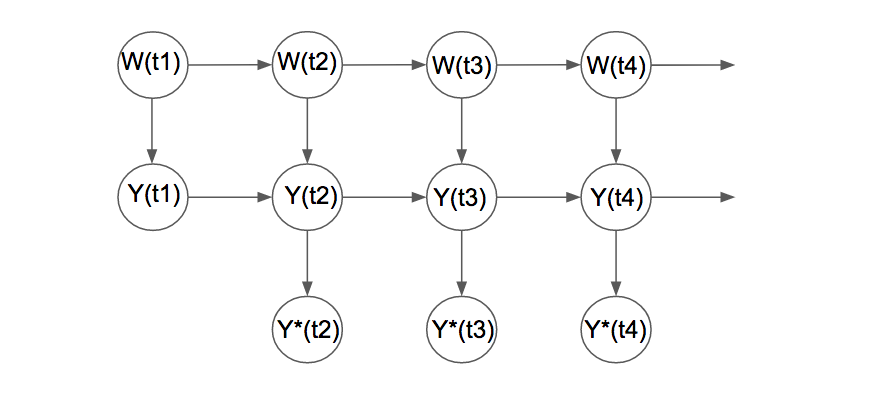
\includegraphics[width=0.6\textwidth]{figures/graphical_rep.png}
\end{figure}
%This provides a model for generating noisy percolation processes.
\begin{itemize}
\item 
$\bm Y^\star = [Y^\star(t_1),...,Y^\star(t_M)]$ --------observed networks
%($t_m^{-}$ represents the most recent transitioning time happened up to observational time $t_m$)
\item 
$\bm Y = [Y(t_1),...,Y(t_M)] $ --------networks in the hidden layer at the observation moments
\item 
$\bm W = [W(t_1),...,W(t_M)] $--------binary rv's in the hidden layer at the observation moments
\item 
$R_{m-1}\in \mathbb{R}$ -------- the total number of augmented transitioning time points between two consecutive observation moments $(t_{m-1},t_{m})$, $t_{m-1}<t_{m}$, $m=2,3...,M$. 
\item 
$\bm \tau^{(m-1)} = [\tau_1^{(m-1)},\tau_2^{(m-1)}, ..., \tau_{R_{m-1}}^{(m-1)}]\in \mathbb{R}^{R_{m-1}}$
-------- the $R_{m-1}$ transition time points between $t_{m-1}$ and $t_{m}$, $m=2,3,...,M$. Let $\tau^{(m-1)}_0 = t_{m-1}$.
\item 
$\bm \tau  = [\bm \tau^{(1)}, \bm \tau^{(2)},...,\bm \tau^{(M-1)}]$ -------- all the augmented transitioning time points from $t_1$ to $t_M$

\item 
$\bm S_{m-1} = (Y(\tau_1^{(m-1)}), Y(\tau_2^{(m-1)}),...,Y(\tau_{R_{m-1}}^{(m-1)})), \bm V_{m-1} =(w(\tau_1^{(m-1)}), w(\tau_2^{(m-1)}),...,w(\tau_{R_{m-1}}^{(m-1)}))$ -------- the sample path from $Y(t_{m-1})$ to $Y(t_m)$ between $t_{m-1}$ and $t_{m}$

\item 
$\bm S = [\bm S_1,\bm S_2,...,\bm S_{M-1}]$ -------- all the augmented networked in the hidden layer at transitioning time points

\item 
$\bm V = [\bm V_1,\bm V_2,...,\bm V_{M-1}]$ -------- all the augmented binary rvs in the hidden layer at transitioning time points
 
\end{itemize}

\subsection{MLE for $\alpha,\beta,p,q,\gamma$}
We propose to estimate $\alpha,\beta,p,q,\gamma$ conditional on the first observation $y^\star(t_1)$, i.e. to maximize the likelihood for the observed data $y^\star(t_2),...,y^\star(t_M)$ conditional on $y^\star(t_1)$. We also assume that at the first observation moment $t_1$: 1) the observed network is noise-free, i.e. $y(t_1)= y^\star(t_1)$; 2) $w(t_1) = 1$. This has the advantage that no distribution assumptions need to be made for the $\big(Y(t_1),W(t_1)\big)$ and $Y^\star(t_1)|Y(t_1)$. So, our goal is to maximize the likelihood for the observed data $y^\star(t_2),...,y^\star(t_M)$ conditional on $y^\star(t_1)$, $y(t_1)$ and $w(t_1)$.

Goal: 
\begin{equation}
\max_{\alpha,\beta,p,q,\gamma} l(\alpha,\beta,p,q,\gamma) = \max_{\alpha,\beta,p,q,\gamma}\log f^c(\bm{y^\star}) =\max_{\alpha,\beta,p,q,\gamma} \log f^c(y^\star(t_1),...,y^\star(t_M))
\end{equation}
where $f^c(\cdot)$ is the conditional pdf for $Y^\star(t_2),...,Y^\star(t_M)$ conditional on $Y^\star(t_1)$.
\subsection{Complete Data MLE}
The log-likelihood for complete data $\bm y^\star$, $\bm y$, $\bm w$ conditional on $y^\star(t_1)$, $y(t_1)$ and $w(t_1)$ is 
\begin{equation}
\begin{split}
l^\star(\alpha,\beta,p,q,\gamma) 
&=\log 
\frac{p(\bm y^\star, \bm y, \bm w )}
{p(y^\star(t_1), y(t_1),w(t_1) )} \\
& = \log p(\bm y^\star, \bm y, \bm w ) - \log p(y^\star(t_1), y(t_1), w(t_1) ) \\
& = \log p(\bm {y^\star}|\bm{y},\bm {w}) 
+ \log p(\bm y, \bm w) -   \log p(y^\star(t_1), y(t_1), w(t_1) )\\
& = \log p(\bm {y^\star}|\bm{y}) 
+ \log p(\bm y, \bm w) -   \log p(y^\star(t_1), y(t_1), w(t_1) ) 
\qquad \text{since } \bm Y^\star \independent \bm W| \bm Y
\\
& = \sum_{m=1}^M \log p(y^\star(t_m)|y(t_m))
+ \log p(\bm y, \bm w) -   \log p(y^\star(t_1), y(t_1), w(t_1) ) 
\qquad \text{since } ddddd \\
&=  \sum_{m=1}^M \log p(y^\star(t_m)|y(t_m))
+ \sum_{m=2}^M\log p(y(t_m), w(t_m)|y(t_{m-1}), w(t_{m-1})) + \log p(y(t_1), w(t_1)) \\
& \qquad - \log p(y^\star(t_1), y(t_1), w(t_1) ) 
\qquad \text{since the Markov property in the hidden layer} \\
&=  \sum_{m=2}^M \log p(y^\star(t_m)|y(t_m))
+ \sum_{m=2}^M\log p(y(t_m), w(t_m)|y(t_{m-1}), w(t_{m-1}))  \\
& \qquad + \log p(y(t_1), w(t_1))+\log p(y^\star(t_m)|y(t_m)) - \log p(y^\star(t_1), y(t_1), w(t_1) ) \\
& =  \sum_{m=2}^M \log p(y^\star(t_m)|y(t_m))
+ \sum_{m=2}^M\log p(y(t_m), w(t_m)|y(t_{m-1}), w(t_{m-1})) 
\end{split}
\end{equation}

\subsubsection{Maximize First Term}
Denote the first term by $f_{\alpha,\beta}(\bm y^\star|\bm y)$, i.e.
\begin{equation}
f_{\alpha,\beta}(\bm y^\star|\bm y) =  \sum_{m=2}^M \log p(y^\star(t_m)|y(t_m)) 
\end{equation}
then 
\begin{equation}
\begin{split}
& \qquad \max_{\alpha,
\beta} \sum_{m=2}^M \log p(y^\star(t_m)|y(t_m)) \\
\end{split}
\end{equation}
\begin{equation}
\log p(y^\star(t_m)|y(t_m)) = ...
\end{equation}
Therefore, we have
 
\begin{equation}
\hat \alpha = 
\end{equation}

\begin{equation}
\hat \beta = 
\end{equation}
\subsubsection{Maximize Second Term}
The second term is the log-likelihood of $y(t_2),...,y(t_M)$, $w(t_2),...,w(t_M)$ conditional on $Y(t_1) =y(t_1), W(t_1)=w(t_1)$. Let $\bm \theta = (p,q,\gamma)$, $\bm y(-t_1) = [y(t_2),...,y(t_M)]$, $\bm w(-t_1) = [w(t_2),...,w(t_M)]$, then the log-likelihood in the second term can be denoted as 
\begin{equation}
\log f_{\bm \theta}(\bm w,\bm y) = \log p_{\bm Y(-t_1), \bm W(-t_1)|Y(t_1),W(t_1)} \big(y(-t_1), \bm w(-t_1)|y(t_1),w(t_1)\big)
=\sum_{m=2}^M\log p_{m-1} \big(y(t_m), w(t_m)|y(t_{m-1}), w(t_{m-1})\big) 
\end{equation}
where $p_{m-1}(\cdot|\cdot) $ is the distribution of $Y(t_m),W(t_m)$ conditional on $Y(t_{m-1}),W(t_{m-1})$, $m=2,...,M$.

The observed data score function conditional on $Y(t_1) =y(t_1), W(t_1)=w(t_1)$ is 
\begin{equation}
\begin{split}
S(\bm \theta; \bm w,\bm y) &= 
\frac{\partial}{\partial \bm \theta} \log f_{\bm \theta}(\bm w,\bm y) \\
& = \frac{\partial}{\partial \bm \theta}\log p_{\bm Y(-t_1), \bm W(-t_1)|Y(t_1),W(t_1)} \big(\bm y(-t_1), \bm w(-t_1) |y(t_1),w(t_1)\big) \\
& = \sum_{m=2}^M \frac{\partial}{\partial \bm \theta} \log p_{m-1}\big(y(t_m), w(t_m)|y(t_{m-1}), w(t_{m-1})\big)  \\
& =  \sum_{m=2}^M S_{m-1}^{obs} (\bm \theta; y(t_m), w(t_m)|y(t_{m-1}), w(t_{m-1})) 
\end{split}
\end{equation}

The total data (observed and augmented data) score function conditional on $Y(t_1) =y(t_1), W(t_1)=w(t_1)$ is 
\begin{equation}
\begin{split}
S_T(\bm \theta; \bm w,\bm y, \bm s, \bm v) &=
\frac{\partial}{\partial \bm \theta} \log f_{\bm \theta}(\bm w,\bm y, \bm s,\bm v)\\
& = \frac{\partial}{\partial \bm \theta}\log p_{\bm Y(-t_1), \bm W(-t_1), \bm S, \bm V|Y(t_1),W(t_1)} \big(\bm y(-t_1), \bm w(-t_1), \bm S, \bm V |y(t_1),w(t_1)\big) \\
& = \sum_{m=2}^M \frac{\partial}{\partial \bm \theta} \log p_{sp}\big(\bm s(t_{m-1}), \bm v(t_{m-1})|y(t_{m-1}), w(t_{m-1})\big)  \\
& =  \sum_{m=2}^M S_{m-1} (\bm \theta;\bm s(t_{m-1}), \bm v(t_{m-1})|y(t_{m-1}), w(t_{m-1})) 
\end{split}
\end{equation}
Notice that $S_{m-1}(\cdot)$ can be calculated for period $t_{m-1}$ to $t_m$ given $\bm s(t_{m-1}), \bm v(t_{m-1}), y(t_{m-1}), w(t_{m-1}), y(t_{m}), w(t_{m})$.


By missing information principle, (prove it???)
\begin{equation}
E(S(\bm \theta; \bm w, \bm y, \bm S, \bm V)|\bm W = \bm w, \bm Y=\bm y) = S(\bm \theta; \bm w, \bm y)
\end{equation}

In order to maximize the second term, 
\begin{equation}
\begin{split}
& \qquad \max_{\bm \theta} \sum_{m=2}^M\log p(y(t_m), w(t_m)|y(t_{m-1}), w(t_{m-1})) \\
& \Leftrightarrow
\text{Solve } S(\bm \theta; \bm w, \bm y) = E(S(\bm \theta; \bm w, \bm y, \bm S, \bm V)|\bm W = \bm w, \bm Y=\bm y) = 0
 \\
\end{split}
\end{equation}













\subsection{Incomplete Data - EM Framework}



\subsubsection*{E-step}
Let $\Gamma =(\alpha,\beta, p,q,\gamma) =(\alpha,\beta, \bm \theta)$, then
\begin{equation}
\begin{split}
 Q(\Gamma; \Gamma^{(n-1}) 
 &= E[\log f_{\Gamma}(\bm w, \bm y, \bm y^\star) |\bm y^\star, \Gamma^{n-1}] \\
& = E[\log f_{\Gamma}(\bm y^\star|\bm y)| \bm y^\star, \Gamma^{n-1}] + E[\log f_{\Gamma}(\bm w, \bm y)| \bm y^\star, \Gamma^{n-1}] 
\end{split}
\end{equation}



\subsubsection*{M-step}

\begin{itemize}




\item First term: \\
\begin{equation}
\begin{split}
E[\log f_{\Gamma}(\bm y^\star|\bm y)| \bm y^\star, \Gamma^{n-1}] &= E( \sum_{m=2}^M \log p(y^\star(t_m)|y(t_m)) | \bm y^\star, \Gamma^{n-1}) \\
& = ddddd...
\end{split}
\end{equation}
has closed-form w.r.t $\alpha, \beta$. Maximizing it w.r.t. $\alpha$, $\beta$ yields the following:

\begin{equation}
\begin{split}
\hat \alpha &= \frac{E[C| \bm y^\star,\Gamma^{n-1}]}
{E[C+D| \bm y^\star,\Gamma^{n-1} ]} \\
\hat \beta & = \frac{E[B| \bm y^\star,\Gamma^{n-1}]}
{E[A+B| \bm y^\star,\Gamma^{n-1} ]} 
\end{split}
\end{equation}





\item Second term: \\
\begin{equation}
\begin{split}
& \qquad \max_{\bm \theta} E[\log f_{\Gamma}(\bm w, \bm y)| \bm y^\star, \Gamma^{n-1}]  \\
 & \Leftrightarrow
 \text{Solve } E[ \frac{\partial}{\partial \bm \theta}
 \log f_{\Gamma}(\bm w, \bm y)| \bm y^\star, \Gamma^{n-1}]  = E[ S(\bm \theta; \bm w,\bm y)| \bm y^\star, \Gamma^{n-1}] =0 \\
& \Leftrightarrow
\text{Solve }
  E \Big[ 
  E \big[ S(\bm \theta; \bm w, \bm y, \bm S, \bm V)|\bm W = \bm w, \bm Y=\bm y \big] 
 |\bm y^\star, \Gamma^{n-1}  \Big] = 0
\end{split}
\end{equation}
So the solution of $E[ S(\bm \theta; \bm w,\bm y)| \bm y^\star, \Gamma^{n-1}] =0$ can be obtained by stochastic approximation via Robbins Monro, at each iteration of which $ S(\bm \theta; \bm w,\bm y)$ can be calculated by taking expectation of the total data score function, i.e. 
$S(\bm \theta; \bm w, \bm y) = E(S(\bm \theta; \bm w, \bm y, \bm S, \bm V)|\bm W = \bm w, \bm Y=\bm y)$. 
\end{itemize}







\section{Algorithm}

\begin{algorithm}[H]
 \KwData{Network snapshots: $\bm y^\star = \big (y^\star(t_1),y^\star(t_2),..., y^\star(t_M) \big)$}
 \KwResult{$\hat \Gamma=[\hat\alpha, \hat \beta, \hat {\bm\theta}] = [\hat\alpha, \hat \beta,\hat p, \hat q, \hat \gamma]$}
 Initialization: $\Gamma^0$\;
 \While{! stopping condition for EM}{
 
   (At $(l+1)^{th}$ EM iteration with current state $\Gamma^{l}= [\alpha^{l}, \beta^{l}, \bm \theta^{l}]$)\\
   
   \While{! stopping condition for Robbins Monro}{
  (At $(b+1)^{th}$ Robbins Monro iteration with current state $\bm \theta_{RM}^{b}$, $\bm \theta_{RM}^{0} = \bm \theta^{l}$)\\
   Sample true network $\bm y^{(b)} = \big(y^{(b)}(t_1),...,y^{(b)}(t_2) \big)$ from $\bm Y|\bm Y^\star = \bm y^\star$ \;
   Get $\bm w^{(b)} =\big(w^{(b)}(t_1),...,w^{(b)}(t_2) \big) $ from $\bm y^{(b)}$\;
   
        \For{$d=1,2,...,D$}{
           Sample sample path $\bm s^{(d)}, \bm v^{(d)}$ from $\bm S,\bm V|\bm W = \bm w^{(b)}, \bm Y = \bm y^{(b)}$\;
           Calculate $S(\bm \theta_{RM}^{b};\bm w^{(b)},\bm y^{(b)},\bm s^{(d)},\bm v^{(d)})$
        }
    Calculate $\hat S(\bm \theta_{RM}^{b};\bm w^{(b)},\bm y^{(b)}) =  \frac{1}{D}\sum_{d=1}^D S(\bm \theta_{RM}^{b};\bm w^{(b)},\bm y^{(b)},\bm s^{(d)},\bm v^{(d)})$\\
    Update $\bm \theta_{RM}^{b+1} = \bm \theta_{RM}^{b} + a_bD^{-1}\hat S(\bm \theta_{RM}^{b};\bm w^{(b)},\bm y^{(b)})$
   }
  Update $\bm \theta^{l+1} = \bm \theta_{RM}^{B+1}$ ($B$ is total number of R-M iterations, i.e. number of particles needed.) 
  Update $\hat \alpha^{l+1}, \hat \beta^{l+1}$ from samples $\bm y_{(0)},\bm y_{(1)},...,\bm y_{(B)} $.
 }
 \caption{EM and Robbins Monro Iterations }
\end{algorithm}














\end{document}



